% Setup - do not change
\documentclass[11pt]{article}
\usepackage[top=0.9in, left=0.9in, bottom=0.9in, right=0.9in]{geometry} 
\usepackage{parskip}

\usepackage[english]{babel}
\usepackage[utf8]{inputenc}
\usepackage{amsmath,amsthm,amssymb,graphicx,pdfpages,lipsum,hyperref}
\usepackage[none]{hyphenat}
\usepackage{csquotes}
\graphicspath{plots}

\setlength\parindent{0pt}
%%%%%%%%%%%%%%%%%%%%%%%%%%%%%%%%%%%%%%%%%%%%%%%%%%%%%%%%%%%%%%%%%%%
% add other packages here if required

%% Bibliography are specified in this file. You can also choose inline bib style if you want to. But make sure your citation style is consistent (and proper)
% For more details on citation: https://library.unimelb.edu.au/recite
\usepackage[sorting = none]{biblatex}
\addbibresource{references.bib}

%%%%%%%%%%%%%%%%%%%%%%%%%%%%%%%%%%%%%%%%%%%%%%%%%%%%%%%%%%%%%%%%%%% the '%' symbol denotes comments
\title{\textbf{Mobility Across America's Concrete Jungle:} \\ Forecasting Yellow Taxi Demand Against Transportation Hubs}
\author{
Izzah Dalila Mohd Khairudin \\
Student ID: 1268317 \\
\href{https://github.com/MAST30034-Applied-Data-Science/mast30034-project-1-duhleelah}{Github repository with commit}
}

\begin{document}
\maketitle

\section{Introduction}
In a bustling metropolitan area like New York City (NYC), maintaining infrastructure such as public transport is crucial to provide accessible travelling for the community, but also mitigate the effects of change in social behaviour. Likewise, significant shifts to urban mobility and routine is an outcome of the COVID-19 pandemic where preferences for commuting via private cars, walking, and cycling has increased substantially \cite{2022urbanmobilitypaper}. Undoubtedly, taxi demand and public transport ridership will be affected by such shift. Hence, this report aims to investigate how the volume of ridership and locations of subway stations affect hourly demand of yellow taxis in NYC.

This analysis will utilise and evaluate unsupervised Machine Learning techniques in predicting the hourly demand by location for yellow taxi trips across NYC. Yellow taxi operators across NYC will benefit from this analysis in allocating their taxis at higher demand areas and locations with less public transportation access. In addition, this investigation will also assist Metropolitan Transportation Authority (MTA) and urban planners in planning future urban infrastructure implementations that can compensate for the appropriate needs of the area.

\subsection{Data Set}
In forming the predictions, the yellow taxi data set from \textbf{TLC Trip Record Data} is utilised \cite{2022YellowTaxiData}. Here, key features such as pick-up and drop off timestamp and locations, passenger count and other payment features are recorded. Other than the yellow taxi being an iconic symbol of NYC, the yellow taxi data was selected upon the basis that it has no travelling restrictions unlike the green or borough taxi. In matching taxi records and locations, the \textbf{TLC Taxi Zone Shapefile} was made use where the boroughs, zones, and boundaries are made not of. 

In assisting the analysis, the \textbf{MTA Subway Hourly Ridership}\cite{SubwayRidership} data set was selected with the understanding of foot traffic at urban mobility hubs like subway stations can be related to the demand of taxi. Key features listed in this data set include hourly ridership, latitude and longitude of subway stations, subway routes, and the borough the station is located, beginning from February 2022 to April 2023. Due to different authoritative bodies, the subway stations and hourly ridership of the Staten Island Railway are not made available which limits the analysis to the remaining four boroughs of NYC. 

The period of analysis chosen is from August 2022 to March 2023. This timeline was selected up to the recent records available from the external data set and for best representation of near future prediction. Furthermore, most COVID restrictions were lifted prior to the selected timeline which is deemed to have little to no significance on the operation of taxis and subways \cite{2021CovidRest}. The following table outlines the shape of the data sets at download.

\begin{center}
\begin{table}[h]
    \centering
    \begin{tabular}{||c|c|c||}
        \hline \textbf{Data set} & \textbf{No. of Instances} & \textbf{No. of Features}\\
        \hline
         TLC Taxi Zone Shapefile & 263 & 7\\
         TLC Yellow Taxi Trip &  26,048,608 & 19 \\
         MTA Subway Hourly Ridership & 5,464,076 & 11 \\
        \hline
    \end{tabular}
    \caption{Shape of selected data sets.}
    \label{table:1}
\end{table}
    
\end{center}

% You can have \section{}, \subsection{}, and \subsubsection{}, \section*{}, \subsection*{}, and \subsubsection*{}
\section{Preprocessing}
Different preprocessing steps were taken to address any anomalies in the three data sets used. Across all data sets, standardising column names to lowercase and changing data types to the most suitable format were performed. 
\subsection{Data Wrangling and Feature Selection}

\subsubsection{TLC Taxi Zone Shapefile}
The taxi zone shapefile required minimal preprocessing due to considerably less features and instances. Apart from the steps performed above, any locations outside of the interest region, particularly Staten Island and Newark Airport, were filtered out of the data set. This is due different authoritative bodies overseeing transportation, as well as the lack of information on stations and ridership in these locations. Features such as shape length and area were removed as the size of a location was not considered as features of interest and to be studied in this analysis. In total, 242 rows of the data set remain, and features such as zone, geometry points, location identifiers and borough were kept.

\subsubsection{TLC Yellow Taxi Trip}
Due to the substantial amount of records (26,048,608 rows) for this data set, many variations and errors for each feature were observed. Multiple approaches were taken to ensure that data quality is preserved to conduct analysis.
\begin{itemize}
    \item \textbf{Dates outside of downloaded timeline} ranging from 2001 to 2009 existed in the data set. Removal of those rows were conducted first and resulted in 26,048,455 rows remaining.
    
    \item \textbf{Locations outside of the interest region} were filtered out of the data set, particularly records with pick up and drop off locations in Staten Island and Newark Airport. Drop offs with location identifiers outside of the specified range by TLC were also found and removed due to the lack of information on these locations. In total, 25,445,920 rows remained.

    \item \textbf{Incorrect pick up and drop off times} where the drop off times are earlier than pick up times, or both pick up and drop off times are the same were discarded from the data set. This resulted in 25,444,247 rows remaining.
    
    \item \textbf{Unusual trip distances} including negative, zero, and unreasonably large values were also found. These rows were discarded, with only distances around 50 miles and below are kept with the notion of the longest distance possible in NYC \cite{NYCDistance}. 25,077,151 rows are remaining after this process.
    
    \item \textbf{Tip amounts} larger than total amounts were found and later discarded under the notion that it cannot exceed the total amount paid, leaving with 24,906,812 rows.

    \item \textbf{Negative or zero fare and total amounts} as well as \textbf{large fare amounts and fees} were also deducted from the data set and deemed faulty records as there is an initial charge of \$2.50 in taxi fare \cite{TLCTaxiFare}. Also, by the logic that passengers are not willing to pay costly taxi fares, a cap of \$500 was set to filter the rows. This leaves 24,902,961 rows.

    \item \textbf{Exceeded values for surcharge columns} were also found and removed as they are fixed by MTA\cite{YellowTaxiDataDict}, leaving 24,893,498 rows.
    
    \item Any zero \textbf{passenger counts} as well as above the lawful limit (maximum 6 passengers) were discovered and discarded from the data set \cite{TLCFAQ}. 23,735,111 remain in the data set.

    \item \textbf{Additional payment and rate code categories} were also found and removed from the given data set, resulting in 23,651,922 rows.
    
\end{itemize}
The data wrangling steps left 23,651,922 rows remaining, approximately 91\% of the rows were retained. As this analysis is focused on location and demand, features that are not related to pick up date, time, location, and passenger count were excluded from the analysis and modelling. These included features related to methods of payment, fees and surcharges, and of boolean or categorical nature. Contextually, it will not provide much information regarding the record. Moreover, features like surcharges have fixed values which will have minimal effect to demand \cite{YellowTaxiDataDict} \cite{TLCUserGuide}. Drop off-related features were also excluded as the analysis is focused on predicting pick up data.

\subsubsection{MTA Subway Hourly Ridership}
The size of the ridership data set is still substantial despite only being a proportion of the taxi data set. The following steps were produced to reach a form of quality data.
\begin{itemize}
    \item \textbf{Features related to station transfers and payment method} were discarded as transfers are a subset of the ridership feature \cite{SubwayDataDict} and payment method is observed to be constant across all instances \cite{SubwayDataDict}. 
    \item \textbf{Code names for boroughs} such as "BX" for Bronx and "M" for Manhattan were recorded in the borough column. This was then imputed with the full name of the borough itself such as "Bronx" and "Manhattan". 
    \item \textbf{Instances outside of specified timeline} were removed as they were not of interest, which resulted in 2,423,609 rows.
\end{itemize}
As no null values or discrepancies were observed in the data exploration phase for this data set, no row filtering was required. In terms of feature selection, only columns of timestamp, ridership, and geometry points of each train station was kept for further analysis. The remaining columns such as station name, routes, and borough were dropped as it can be inferred from the TLC Taxi Zone Shapefile.

\subsection{Feature Engineering and Data Aggregation}
Across both data sets, features of time such as year, month, day of the week, day of the month, and hour were extracted from the timestamp. 

For the TLC Taxi Data, the data set is first grouped by the location identifier and time features to obtain the number of hourly pick ups as well as the number of hourly passengers. As for subway ridership, the point geometry of each station is checked against the polygon geometry of the TLC Taxi Zone Shapefile. This is then merged with the aggregated subway data where to obtain the hourly ridership of a location, it was grouped by the station and timestamp.

In order to obtain both hourly pick ups and ridership, the yellow taxi and subway ridership data is then merged on location identifier and time-related columns. For ease of training, the resulting data set is separated into two, 2022 and 2023, for training and testing purposes.

\section{Analysis and Geospatial Visualisation}
Analysis on the cleaned data sets and the trends between the interested attributes are explored in this part of the report. 

\subsection{Total Pick Ups and Ridership}
In Figure 1, the logarithm of total pick ups are mapped against the location identifiers of NYC, due to the large difference between pick ups in each area. It is evident that the Manhattan borough and JFK Airport are heaviest with taxi pick ups. This may suggest the inflow of tourists as famous tourist destinations in NYC are densely populated.

\begin{figure}[ht]
    \centering
    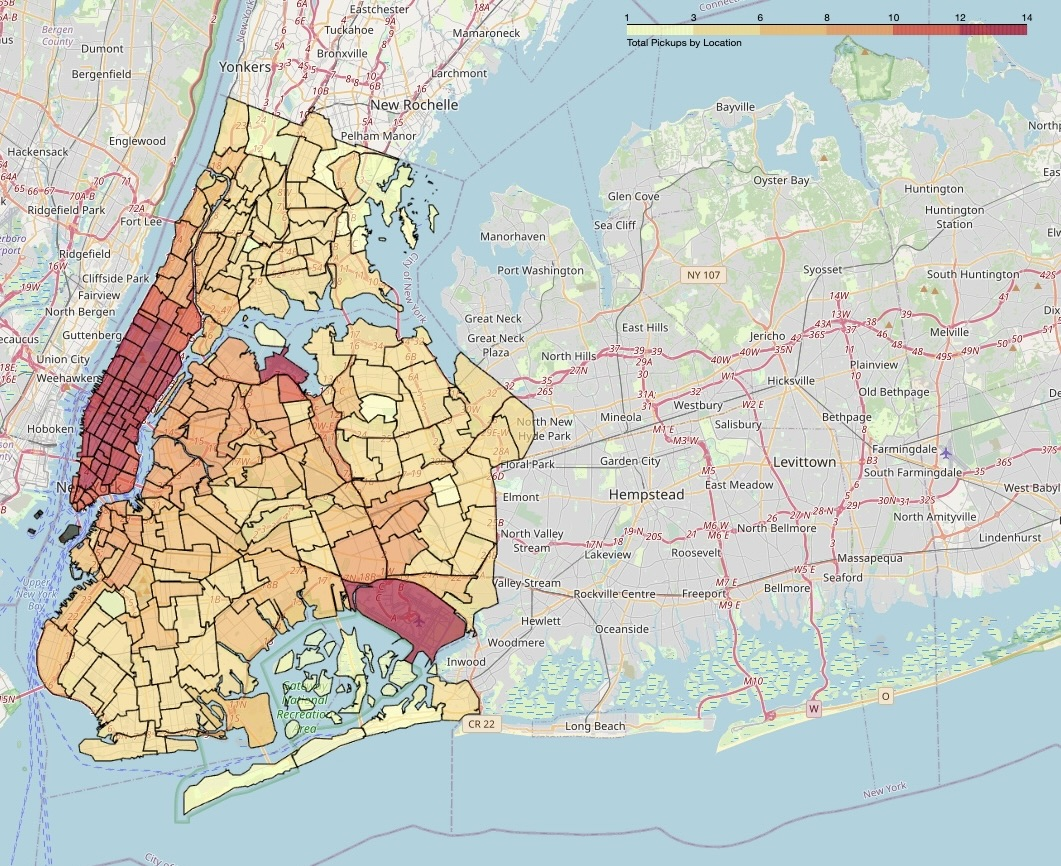
\includegraphics[width=0.45\textwidth]{plots/NYC Total Pickups.jpeg}
    \caption{The log of total taxi pick ups in NYC between August 2022 to March 2023} % refer to this image as (Figure 1)
    \centering
\end{figure}

\begin{figure}
    \centering
    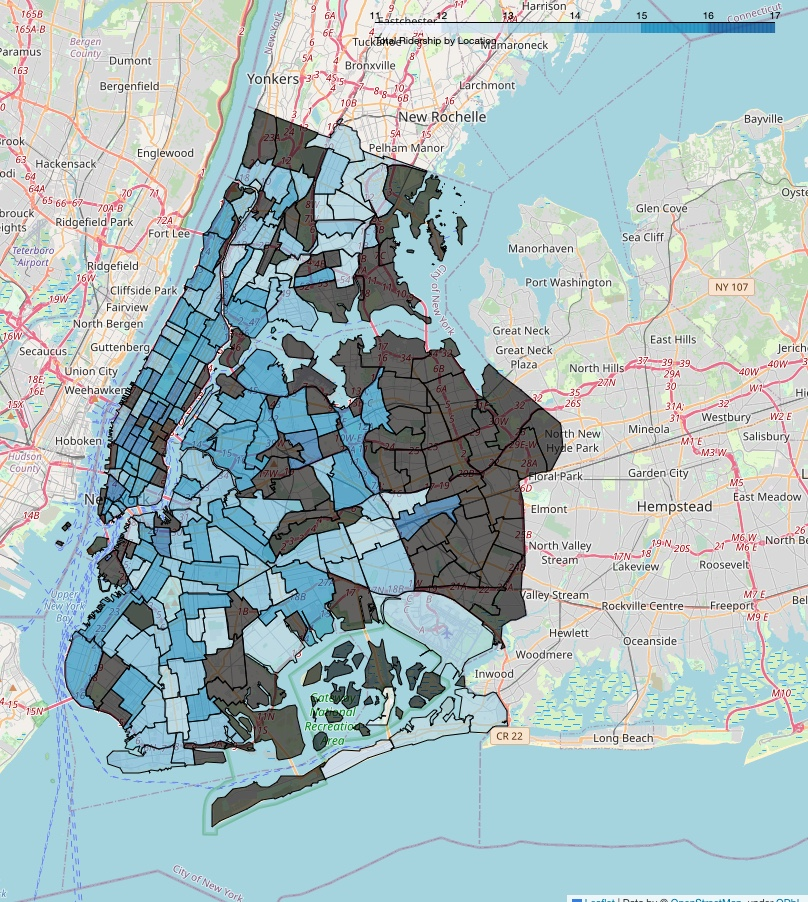
\includegraphics[width=0.45\textwidth]{plots/NYC Total Ridership.jpeg}
    \caption{The log of total hourly riderships in NYC between August 2022 to March 2023} % refer to this image as (Figure 2)
    \centering
\end{figure}

As for Figure 2, it depicts the logarithm of the hourly ridership in NYC. Upon face-value, the inner-west areas of NYC tends to be more concentrated in population flow. Same as Figure 1, a trend in an inflow towards more tourist destinations such as Times Square, Brooklyn Bridge, and Statue of Liberty is observed. Furthermore, areas along the east of NYC spectated lower taxi pick up rates and zero subway ridership. This may suggest the lack of subway infrastructure in these regions are no riderships were recorded during the 8-month timeline. 

\subsection{Trends in Hourly Movement}
In the analysis, there is a clear distinction between hourly taxi pickup demand, whereby peak hours range between 4-7 pm every day. On the flip side, demand is at an all time low at 5 am across all weekdays. This may be reflective of the routine of the NYC population whereby evening commutes occur more frequently more than morning commutes.

\section{Modelling}
To predict the hourly pick ups of taxi demand, two different regression models have been deployed. This section will introduce the concepts behind the model and its relevance to the data sets.

\subsection{Ridge Regression}
Ridge regression is a derivative of the linear regression model where it is ideal for columns with multicollinearity and to prevent overfitting \cite{RidgeReg}. As this data set involves co-dependence between date columns and how pick ups and ridership vary hourly, this model was adopted. 
\subsection{Decision Tree Regressor}
Decision tree regressor is a supervised learning algorithm that performs predictions of continuous values by splitting its root into multiple nodes, and splits into multiple depths. Ultimate each branch or path taken by this algorithm determines the predicted value \cite{DTReg}.
\section{Discussion}
Table 2 outlines the metrics of both supervised regression models in predicting the hourly taxi demand in NYC.

The results suggest that minimal errors have been made across both models, whereby a low MSE is recorded for both models. This is supported by the high R2 score for both ridge regression and decision tree regression where a good-fit is detected from the use of this model. However, this may also be an indication of overfitting towards the data set as the scores of MSE are minute in decimal places and R2 scores are almost close to 1. 

\begin{center}
\begin{table}[h]
    \centering
    \begin{tabular}{||c|c|c||}
        \hline \textbf{Metrics} & \textbf{Ridge Regression} & \textbf{Decision Tree Regression}\\
        \hline
         Validation R2 score & 0.9999999999999999 & 0.9999996860123411\\
         Validation MSE score & 1.8839294549516947e-13 & 0.0010435229334232368\\
         Test R2 score &  0.9999999999999999 & 0.9999883921310759 \\
         Test MSE value & 2.071222498452769e-13 & 0.03891736755465362 \\
        \hline
    \end{tabular}
    \caption{Evaluation Metrics of Two Regression Models}
    \label{table:1}
\end{table}
    
\end{center}

\section{Recommendations}
From the analysis in section 3, there is an apparent trend of lesser pick ups and riderships along the Northeast of NYC. This may be indicative to urban planners that more public infrastructure can be built and facilitated within these less populated areas as it may assist in removing congestion along the inner-west of the city. On the other hand, industrial areas can be located to these low populated areas as to maximise utilisation of space in a compact city like New York. 

Taxi drivers should continue to focus on busy areas such as Manhattan and the airport. This will prolong their benefits as seen in Figures 1 and 2, and as the tourist destinations in NYC continue to be a crowded destination.
\section{Conclusion}
In summary, methods of analysis and learning such as ridge regression and decision tree regression were briefly touched upon in exploring the prediction of hourly pick up taxi demands in NYC against the subway ridership trends and its past data. The results of the prediction metrics above suggest that a relationship exists between the hourly ridership volume and taxi demand in NYC, and that future avenues by the NYC urban planners can be pursued to improve the city's infrastructure.

Moving forward, more in-depth analysis on the taxi pick ups and other public transport within each borough can be conducted to develop a deeper understanding of the patterns of NYC commute. With that, exploring different regression models can help widen understanding from different aspects of the problem.

\clearpage

% BEGIN REFERENCES SECTION
\printbibliography
\end{document}